\documentclass[a4paper,11pt]{article}

\usepackage[left=1in,right=1in,top=3cm,bottom=3cm]{geometry}

\usepackage{graphicx}
\usepackage{xcolor}
\begin{document}
Problem description:

A cat runs along a straight line with a constant speed $v_c$.
A Dog runs towards the cat with speed $v_d$.
\begin{center}
    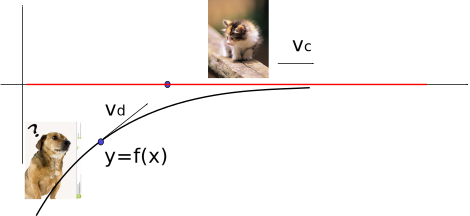
\includegraphics[width=.7\textwidth]{run.pdf}
\end{center}

Try to set up  formulae to describe the curve that the dog runs.
  \begin{center}------------------------\end{center}

\noindent Solution:~\\

For mathematical simplicity, we invert coordinates $x$ and $y$, ie. the cat
runs along the $y$ axis. Therefore, at time $t$, the positions of cat and
dog are (0, $v_c t$) and ($x$, $y$) respectively. Thus we have:
\begin{equation}\label{eq1}
    y' = \frac{y-v_c t}{x}
\end{equation}

At point ($x$, $y$), the dog has moved $s=\displaystyle{\int}\sqrt{1+(y')^2} dx = v_d t$. Thus:
\begin{equation}\label{eq2}
    t = \frac{1}{v_d}\int \sqrt{1+(y')^2} dx
\end{equation}

Replace $t$ in eq.(\ref{eq1}):
\begin{equation}\label{eq3}
    xy' = y - \frac{v_c}{v_d}\int \sqrt{1+(y')^2}dx
\end{equation}

Differentiating both side, we have:
\begin{equation}\label{eq4}
    xy'' = -\frac{v_c}{v_d} \sqrt{1+(y')^2}
\end{equation}
Let $u=y'$, then $y''=\displaystyle{\frac{du}{dx}}$.
Eq(\ref{eq4}) becomes:
\begin{equation}\label{eq5}
    x \frac{du}{dx} = -\frac{v_c}{v_d} \sqrt{1+u^2}
\end{equation}
\begin{equation}\label{eq6}
    \frac{du}{\sqrt{1+u^2}} = -\frac{v_c}{v_d} \frac{dx}{x}
\end{equation}
\begin{equation}\label{eq7}
    \ln |u + \sqrt{1+u^2}| = -\frac{v_c}{v_d}\ln|x| + C'_1
\end{equation}
\begin{equation}\label{eq8}
    u + \sqrt{1+u^2} = -C_1 x^{-v_c/v_d}
\end{equation}
\begin{equation}\label{eq9}
    u = \frac{1- C_1^2 x^{-2v_c/v_d}}{2C_1 x^{-v_c/v_d}}
    = \frac{1}{2C_1} x^{v_c/v_d} - \frac{C_1}{2} x^{-v_c/v_d} = \frac{dy}{dx}
\end{equation}
\begin{equation}\label{eq10}
    y = \left\{ \begin{array}{l}
        \displaystyle{\frac{1}{4C_1} x^2 -\frac{C_1}{2}\ln |x|}+C_2,
            v_c=v_d\\
        \displaystyle{\frac{1}{2C_1(v_c/v_d+1)} x^{v_c/v_d+1} +
        \frac{C_1}{2(v_c/v_d-1)}x^{1-v_c/v_d}} +C_2, v_c\ne v_d
    \end{array}
    \right.
\end{equation}


Assume initial conditions ($t=0$): cat at (0, 0), dog at ($L$, 0).
At this moment, $y'=u=0$. Plugging $u=0, x=L$ into eq.(\ref{eq8}),
$C_1$ can be calculated:

\begin{equation}\label{eq11}
    C_1 = -L^{v_c/v_d}
\end{equation}

Then put $x=l, y=0$ into eq.(\ref{eq10}) to calculate $C_2$:

\begin{equation}\label{eq12}
    C_2 = \left\{ \begin{array}{l}
        \displaystyle{\frac{C_1}{2}\ln L - \frac{L^2}{4C_1}}, v_c=v_d\\
        -\displaystyle{\frac{L^{v_c/v_d+1}}{2C_1(v_c/v_d+1)}
        -\frac{C_1 L^{1-v_c/v_d}}{2(v_c/v_d-1)}}, v_c\ne v_d
    \end{array}
    \right.
\end{equation}

\ \\ \ \\

\noindent \textcolor{red}{MORE EXERCISE: Try to draw the curve using MATLAB.
\ \\
Assume $v_c$=5m/s, $v_d$=5m/s, $L$=50 m.}

\end{document}
